% !TEX TS-program = pdflatexmk
% !TEX program = pdflatex
% Typeset in TeXShop, or run make problem HW=hw03 from the repository root.
% Based on problems/template.tex; the template is unchanged.
% Source: HW3 Intro to Math Analysis I (1).pdf, pages 1--2.
% MA-GY-6213, Homework No. 3, due Friday 10/2/2026.
% Eight questions; no solutions were supplied with the assignment.
% The source's Week 3 topic summary is metadata, not additional exercises.
\documentclass[nohyper,nobib,nofonts]{tufte-handout}
% Resolve shared inputs from either the repository root or problems/.
\newcommand{\analysisroot}{..}
\IfFileExists{preamble.tex}{\renewcommand{\analysisroot}{.}}{}
\makeatletter
\edef\input@path{{\analysisroot/}}
\makeatother
% Shared packages and typography for the book and homework handouts.
% Handouts set this directory when TeXShop compiles from problems/.
\providecommand{\analysisroot}{.}
\usepackage[T1]{fontenc}
% Give titletoc a separate part number before nameref wraps \@part.
\usepackage{etoolbox}
\makeatletter
\@ifclassloaded{tufte-book}{%
  \patchcmd{\@part}
    {\thepart\hspace{1em}}
    {\protect\numberline{\thepart}}
    {}
    {\PackageError{analysis-notes}{Could not format part contents labels}
      {Check the book class definition of \string\@part.}}
}{}
\makeatother

\usepackage{nameref}
\usepackage{amsmath,amssymb,amsthm}
\usepackage{aliascnt}
\usepackage{graphicx}
\usepackage{tikz}
\usetikzlibrary{arrows.meta}
\usepackage{booktabs}
\usepackage{multicol} % Formula sheet and multicolumn specimen examples.
\usepackage{needspace} % Keep a section opening together when space is short.
% Packages used by the temporary Tufte specimen content.
\usepackage{fancyvrb,xspace,units,makeidx}
\fvset{fontsize=\small}
\usepackage{url}
\usepackage{lipsum} % Remove after all placeholder prose has been replaced.
% AMS numeric references, alphabetised by author, using the AMS's own style.
% Keep the resource path relative so handouts also build from problems/.
\usepackage[numbers,sort&compress]{natbib}
\bibliographystyle{amsplain}
\newcommand{\analysisbibliography}{%
  % A leading ./ prevents BibTeX from using latexmk's adjusted search path
  % when it changes into build/. Direct problems/ builds need ../ instead.
  \ifthenelse{\equal{\analysisroot}{.}}%
    {\bibliography{bibliography}}%
    {\bibliography{../bibliography}}%
}

\graphicspath{{\analysisroot/figures/}}
\setkeys{Gin}{width=\linewidth,totalheight=\textheight,keepaspectratio}
\setcounter{secnumdepth}{1}

% Retain the borrowed title/contents design only for the book.
% Adapted from Kevin Godby's Tufte-LaTeX title/contents example:
% https://groups.google.com/forum/#!topic/tufte-latex/ujdzrktC1BQ
\makeatletter
\@ifclassloaded{tufte-book}{%
  \makeindex
  % Leave room for two-digit appendix figure numbers such as C.13.
  \patchcmd{\@tufte@lof@line}{\@tempdima 2.0em}{\@tempdima 3.0em}
    {}
    {\PackageError{analysis-notes}{Could not widen list-of-figures numbers}
      {Check the Tufte list-of-figures definition.}}
  \setcounter{tocdepth}{0} % Parts and chapters only.
  % Title-only chapter headings; retain counters for sections and references.
  \titleformat{\chapter}[block]
    {\relax\ifthenelse{\NOT\boolean{@tufte@symmetric}}{\begin{fullwidth}}{}}
    {}
    {0pt}
    {\huge\rmfamily\itshape}
    [\ifthenelse{\NOT\boolean{@tufte@symmetric}}{\end{fullwidth}}{}%
      % The fullwidth list must not overwrite the chapter's paragraph hook.
      % Otherwise the first section can lose its normal space after prose.
      \@endpefalse]
  \renewcommand{\maketitlepage}{%
    \begingroup
    \setlength{\parindent}{0pt}
    {\fontsize{24}{24}\selectfont\textit{\@author}\par}
    \vspace{1.75in}
    \begin{fullwidth}
      \raggedright
      {\fontsize{36}{44}\selectfont\@title\par}
    \end{fullwidth}
    \vspace{0.5in}
    {\fontsize{14}{14}\selectfont\textsf{\smallcaps{\@date}}\par}
    \vfill
    {\fontsize{14}{14}\selectfont\textit{\@publisher}\par}
    \thispagestyle{empty}
    \endgroup
  }
  \titlecontents{part}
    [0pt]
    {\addvspace{0.75\baselineskip}\normalfont\normalsize}
    {\allcaps{Part~\thecontentslabel}\quad\allcaps}
    {\allcaps}
    {}
    [\vspace{0.5\baselineskip}]
  % Hide chapter numbers in the contents as well.
  \titlecontents{chapter}
    [4em]
    {\normalfont\normalsize}
    {\textit}
    {\textit}
    {\qquad\thecontentspage}
    [\vspace{0.5\baselineskip}]
}{}
\makeatother

% Enable book and handout links after the Tufte contents customizations.
% The classes' nohyper option defers loading; keep sidenotes unlinked.
\makeatletter
\usepackage[hidelinks,hyperfootnotes=false,bookmarksdepth=0]{hyperref}
% Tufte's pre-expanded author can contain fragile formatting commands.
% Let hyperref strip formatting from the unexpanded author for PDF metadata.
\pdfstringdefDisableCommands{\let\thanklessauthor\@author}
% One caption convention for the book and homework handouts. Load after
% hyperref, and explicitly retain Tufte's margin typography and alignment.
\usepackage{caption}
\DeclareCaptionFont{tufte}{\@tufte@caption@font}
\DeclareCaptionJustification{tufte}{\@tufte@caption@justification}
\captionsetup{
  font=tufte,labelfont=bf,labelsep=period,
  justification=tufte,singlelinecheck=false,parindent=0pt,
  % Tufte builds captions in separate margin boxes; link to the caption.
  hypcap=false
}
\makeatother

% Arrange margin content as a page-sized column, keeping captions with figures.
% https://ctan.org/pkg/marginfix
\usepackage{marginfix}
\usepackage{zref-savepos}
\setlength{\marginparpush}{12pt}
\setlength{\marginheightadjustment}{-6pt}
\makeatletter
\@ifclassloaded{tufte-book}{%
  % Decide a break before starting the heading and its margin insertion.
  \AtBeginDocument{%
    \BeforeBeginEnvironment{exercise}{\Needspace{3\baselineskip}}%
  }
  % Solution links need the final heading baseline, rather than marginfix's
  % page-height estimate, which omits later vertical stretching and floats.
  \let\analysis@marginlabel\@empty
  \newcommand{\analysissolutionnote}[2]{%
    \begingroup
      \edef\analysis@marginlabel{analysis-solution-#1}%
      \leavevmode\zsavepos{\analysis@marginlabel}%
      \marginnote{#2}%
    \endgroup
  }
  % Associate the saved position with both allocated note boxes. Other notes
  % clear the association when LaTeX reuses those boxes.
  \pretocmd{\@xympar}{%
    \expandafter\xdef\csname analysis@marginlabel@\number\@marbox\endcsname
      {\analysis@marginlabel}%
    \expandafter\xdef\csname analysis@marginlabel@\number\@currbox\endcsname
      {\analysis@marginlabel}%
  }{}{\PackageError{analysis-notes}{Could not track solution margin boxes}
    {Check the LaTeX margin paragraph definition.}}
  \let\analysis@margin@getypos\MFX@getypos
  % Record the actual top of each margin column, including pages with top floats.
  \patchcmd{\MFX@attachmargin}{\if\MFX@leftmargin}{%
    \zsavepos{analysis-margin-top-\thepage}%
    \if\MFX@leftmargin
  }{}{\PackageError{analysis-notes}{Could not locate the margin column}
    {Check the marginfix margin attachment definition.}}
  \renewcommand{\MFX@getypos}{%
    \analysis@margin@getypos
    \ifcsname analysis@marginlabel@\number\@marbox\endcsname
      \edef\analysis@label{%
        \csname analysis@marginlabel@\number\@marbox\endcsname}%
      \ifx\analysis@label\@empty\else
        \ifnum\zposy{\analysis@label}>0\relax
          \ifnum\zposy{analysis-margin-top-\thepage}>0\relax
            \dimen@\dimexpr\zposy{analysis-margin-top-\thepage}sp
              -\zposy{\analysis@label}sp-\ht\@marbox\relax
            \edef\mfx@ypos{\the\dimen@}%
          \fi
        \fi
      \fi
    \fi
  }
}{}
% Treat offsets as preferred positions, not whitespace inside the measured box.
% Negative internal space can hide occupied height from the margin scheduler.
\renewcommand{\marginnote}[2][0pt]{%
  \ifthenelse{\boolean{@tufte@loadnatbib}}{%
    \let\cite\@tufte@infootnote@cite
  }{}%
  \gdef\@tufte@citations{}%
  \mparshift{#1}%
  \marginpar{%
    \@tufte@marginnote@font\@tufte@marginnote@justification
    \@tufte@margin@par\noindent #2%
  }%
  \@tufte@print@citations
  \ifthenelse{\boolean{@tufte@loadnatbib}}{%
    \let\cite\@tufte@normal@cite
  }{}%
}
\renewenvironment{@tufte@margin@float}[2][-1.2ex]
  {\FloatBarrier
    \def\analysis@margin@offset{#1}%
    \begin{lrbox}{\@tufte@margin@floatbox}%
      \begin{minipage}[t]{\marginparwidth}%
        \@tufte@caption@font
        \def\@captype{#2}%
        \@tufte@caption@justification
        \@tufte@margin@par\noindent
  }
  {\end{minipage}%
    \end{lrbox}%
    \ifdim\dimexpr\ht\@tufte@margin@floatbox+\dp\@tufte@margin@floatbox\relax
        <\dimexpr\textheight+\marginheightadjustment\relax
      \mparshift{\analysis@margin@offset}%
      \marginpar{\usebox{\@tufte@margin@floatbox}}%
    \else
      \PackageError{analysis-notes}{Margin float is taller than the usable margin}
        {Use a main-text figure or table instead; keep labels readable.}%
    \fi
  }
% Keep Tufte's standard height handling for ordinary and full-width floats.
% Their margin captions must not reserve vertical space in the main text.
\makeatother

% Shared notation and environments. Keep topic-specific macros local.
\newcommand{\N}{\mathbb{N}}
\newcommand{\Z}{\mathbb{Z}}
\newcommand{\Q}{\mathbb{Q}}
\newcommand{\R}{\mathbb{R}}
\newcommand{\C}{\mathbb{C}}

% Draft additions awaiting the author's review. Keep ordinary result styles.
% Remove the wrapper after approval to restore the surrounding text colour.
\definecolor{pendingreviewcolor}{HTML}{486581}
\newenvironment{pendingreview}{%
  \par\color{pendingreviewcolor}%
}{\par}
\newcommand{\pendingreviewtext}[1]{\textcolor{pendingreviewcolor}{#1}}

% One convention for named, linked cross-references in every document.
\renewcommand*{\figureautorefname}{Figure}
\renewcommand*{\tableautorefname}{Table}
\renewcommand*{\partautorefname}{Part}
\renewcommand*{\chapterautorefname}{Chapter}
\renewcommand*{\appendixautorefname}{Appendix}
\renewcommand*{\sectionautorefname}{\S}
\renewcommand*{\subsectionautorefname}{\S}
\renewcommand*{\subsubsectionautorefname}{\S}
\renewcommand*{\theoremautorefname}{Theorem}
% Hyperref appends ~, the reference number, and \null to the name.
% Consume that number here to retain the usual equation parentheses.
\def\equationautorefname~#1\null{Equation~(#1)\null}

% Keep submission-specific layout hints out of shared book exercises.
\makeatletter
\newcommand{\handoutonly}[1]{\@ifclassloaded{tufte-handout}{#1}{}}
% The handouts print solutions immediately; only the book needs these links.
\newcommand{\solutionlink}[1]{%
  \@ifclassloaded{tufte-book}{%
    \analysissolutionnote{#1}{%
      \hyperref[sol:#1]{Solution on page~\pageref*{sol:#1}.}}%
  }{}%
}
\makeatother

% Select the original exercise number for the next appendix restatement.
\newcommand{\restatedexercisekey}{}
\newcommand{\solutionheading}[1]{%
  \renewcommand{\restatedexercisekey}{#1}%
}

% Reuse the exercise's theorem styling and original number. Register only
% the solution anchor, not a second exercise label or solution margin link.
\newenvironment{restatedproblem}{%
  \let\restatedproblemlabel\label
  \renewenvironment{exercise}{%
    \begin{restatedexercise}%
    \phantomsection
    \restatedproblemlabel{sol:\restatedexercisekey}%
  }{\end{restatedexercise}}%
  \renewcommand{\label}[1]{}%
  \renewcommand{\solutionlink}[1]{}%
}{\par}

% Publication month and year used on the copyright page.
\newcommand{\monthyear}{%
  \ifcase\month\or January\or February\or March\or April\or May\or June\or
  July\or August\or September\or October\or November\or December\fi
  \space\number\year
}

% One shared counter makes results unambiguous within each section.
% Alias counters let autoref identify the kind of result, not just its number.
\newcommand{\newsharedtheorem}[2]{%
  \newaliascnt{#1}{theorem}%
  \newtheorem{#1}[#1]{#2}%
  \aliascntresetthe{#1}%
  % Follow later changes to the theorem format, including handout numbering.
  \expandafter\renewcommand\csname the#1\endcsname{\thetheorem}%
  \expandafter\providecommand\csname #1autorefname\endcsname{#2}%
}
\theoremstyle{plain}
\newtheorem{theorem}{Theorem}[section]
\newsharedtheorem{lemma}{Lemma}
\newsharedtheorem{proposition}{Proposition}
\newsharedtheorem{corollary}{Corollary}
\newtheorem*{conjecture}{Conjecture}
\theoremstyle{definition}
\newsharedtheorem{definition}{Definition}
\newsharedtheorem{property}{Property}
\newsharedtheorem{example}{Example}
\newsharedtheorem{exercise}{Exercise}
\newtheorem*{restatedexercise}{\autoref{ex:\restatedexercisekey}}
\theoremstyle{remark}
\newsharedtheorem{remark}{Remark}

% Catalogue numbered theorem statements using their existing counters and
% hyperlink anchors. Match the book's figure/table list formatting.
\makeatletter
\@ifclassloaded{tufte-book}{%
  \newcommand{\listoftheorems}{%
    \begingroup
    % Begin directly after the tables, without a blank facing page.
    \let\cleardoublepage\clearpage
    \chapter*{List of Theorems}%
    \@starttoc{loe}%
    \endgroup
  }
  \let\l@theorem\@tufte@lof@line
  \providecommand*{\toclevel@theorem}{2}
}{}
% Scan this patch directly so etoolbox can handle its parameter characters.
\ifdefined\listoftheorems
  \pretocmd{\@begintheorem}{%
    \ifstrequal{#1}{Theorem}{%
      \ifblank{#2}{}{%
        \addcontentsline{loe}{theorem}{\protect\numberline{#2}#3}%
      }%
    }{}%
  }{}{%
    \PackageError{analysis-notes}{Could not register theorem list entries}
      {Check the amsthm definition of \string\@begintheorem.}%
  }
\fi
\makeatother

% BEGIN TUFTE PLACEHOLDER HELPERS
% Adapted from the supplied Tufte-LaTeX sample (Apache-2.0).
% Remove these documentation helpers once the specimens are replaced.
\newcommand{\hangp}[1]{\makebox[0pt][r]{(}#1\makebox[0pt][l]{)}}

%%
% Prints an asterisk that takes up no horizontal space.
% Useful in tabular environments.

%%
% Prints a trailing space in a smart way.


%%
% Some shortcuts for Tufte's book titles.  The lowercase commands will
% produce the initials of the book title in italics.  The all-caps commands
% will print out the full title of the book in italics.
\newcommand{\vdqi}{\textit{VDQI}\xspace}
\newcommand{\ei}{\textit{EI}\xspace}
\newcommand{\ve}{\textit{VE}\xspace}
\newcommand{\be}{\textit{BE}\xspace}
\newcommand{\VDQI}{\textit{The Visual Display of Quantitative Information}\xspace}
\newcommand{\EI}{\textit{Envisioning Information}\xspace}
\newcommand{\VE}{\textit{Visual Explanations}\xspace}
\newcommand{\BE}{\textit{Beautiful Evidence}\xspace}

\newcommand{\TL}{Tufte-\LaTeX\xspace}

% Typesets the font size, leading, and measure in the form of 10/12x26 pc.
\newcommand{\measure}[3]{#1/#2$\times$\unit[#3]{pc}}

% Macros for typesetting the documentation
\newcommand{\hlred}[1]{\textcolor{Maroon}{#1}}% prints in red
\newcommand{\hangleft}[1]{\makebox[0pt][r]{#1}}
\newcommand{\hairsp}{\hspace{1pt}}% hair space
\newcommand{\hquad}{\hskip0.5em\relax}% half quad space
\newcommand{\ie}{\textit{i.\hairsp{}e.}\xspace}
\newcommand{\eg}{\textit{e.\hairsp{}g.}\xspace}
\newcommand{\na}{\quad--}% used in tables for N/A cells
\providecommand{\XeLaTeX}{X\lower.5ex\hbox{\kern-0.15em\reflectbox{E}}\kern-0.1em\LaTeX}
\newcommand{\tXeLaTeX}{\XeLaTeX\index{XeLaTeX@\protect\XeLaTeX}}
% \index{\texttt{\textbackslash xyz}@\hangleft{\texttt{\textbackslash}}\texttt{xyz}}
\newcommand{\tuftebs}{\symbol{'134}}% a backslash in tt type in OT1/T1
\newcommand{\doccmdnoindex}[2][]{\texttt{\tuftebs#2}}% command name -- adds backslash automatically (and doesn't add cmd to the index)
\newcommand{\doccmddef}[2][]{%
  \hlred{\texttt{\tuftebs#2}}\label{template:cmd:#2}%
  \ifthenelse{\isempty{#1}}%
    {% add the command to the index
      \index{#2 command@\protect\hangleft{\texttt{\tuftebs}}\texttt{#2}}% command name
    }%
    {% add the command and package to the index
      \index{#2 command@\protect\hangleft{\texttt{\tuftebs}}\texttt{#2} (\texttt{#1} package)}% command name
      \index{#1 package@\texttt{#1} package}\index{packages!#1@\texttt{#1}}% package name
    }%
}% command name -- adds backslash automatically
\newcommand{\doccmd}[2][]{%
  \texttt{\tuftebs#2}%
  \ifthenelse{\isempty{#1}}%
    {% add the command to the index
      \index{#2 command@\protect\hangleft{\texttt{\tuftebs}}\texttt{#2}}% command name
    }%
    {% add the command and package to the index
      \index{#2 command@\protect\hangleft{\texttt{\tuftebs}}\texttt{#2} (\texttt{#1} package)}% command name
      \index{#1 package@\texttt{#1} package}\index{packages!#1@\texttt{#1}}% package name
    }%
}% command name -- adds backslash automatically
\newcommand{\docopt}[1]{\ensuremath{\langle}\textrm{\textit{#1}}\ensuremath{\rangle}}% optional command argument
\newcommand{\docarg}[1]{\textrm{\textit{#1}}}% (required) command argument
\newenvironment{docspec}{\begin{quotation}\small\ttfamily\parskip0pt\parindent0pt\ignorespaces}{\end{quotation}}% command specification environment
\newcommand{\docenv}[1]{\texttt{#1}\index{#1 environment@\texttt{#1} environment}\index{environments!#1@\texttt{#1}}}% environment name
\newcommand{\docenvdef}[1]{\hlred{\texttt{#1}}\label{template:env:#1}\index{#1 environment@\texttt{#1} environment}\index{environments!#1@\texttt{#1}}}% environment name
\newcommand{\docpkg}[1]{\texttt{#1}\index{#1 package@\texttt{#1} package}\index{packages!#1@\texttt{#1}}}% package name
\newcommand{\doccls}[1]{\texttt{#1}}% document class name
\newcommand{\docclsopt}[1]{\texttt{#1}\index{#1 class option@\texttt{#1} class option}\index{class options!#1@\texttt{#1}}}% document class option name
\newcommand{\docclsoptdef}[1]{\hlred{\texttt{#1}}\label{template:clsopt:#1}\index{#1 class option@\texttt{#1} class option}\index{class options!#1@\texttt{#1}}}% document class option name defined
\newcommand{\docmsg}[2]{\bigskip\begin{fullwidth}\noindent\ttfamily#1\end{fullwidth}\medskip\par\noindent#2}
\newcommand{\docfilehook}[2]{\texttt{#1}\index{file hooks!#2}\index{#1@\texttt{#1}}}
\newcommand{\doccounter}[1]{\texttt{#1}\index{#1 counter@\texttt{#1} counter}}
% END TUFTE PLACEHOLDER HELPERS

% Shared physical dimensions for interval and number-line diagrams.
\tikzset{
  interval diagram/.style={
    x=1cm,y=6mm,font=\footnotesize,
    color=black,line width=0.5pt,line cap=round,line join=round,
    >={Stealth[length=4pt,width=3pt]}
  },
  interval endpoint/.style={
    circle,draw=black,line width=0.5pt,
    minimum size=4pt,inner sep=0pt,outer sep=0pt
  },
  interval open/.style={interval endpoint,fill=white},
  interval closed/.style={interval endpoint,fill=black},
  interval label/.style={inner sep=1pt}
}


% Preserve the original question numbers independently of book numbering.
\renewcommand{\thetheorem}{\arabic{theorem}}

\title{Homework 03}
\author[Lucas Barbosa, lc6424]{Lucas Barbosa, \texttt{lc6424}}
\date{Due Friday, October 2, 2026}

\begin{document}
\maketitle

% !TEX root = ../../hw03.tex
% Source: HW3 Intro to Math Analysis I (1).pdf, page 1, question 1.
\begin{exercise}
  \label{ex:hw03:dedekind-infimum}
  Use the existence of the Dedekind cut in $\R$ to prove the greatest lower
  bound property. That is, if $S$ is a nonempty subset of $\R$ which is
  bounded below, then there is a unique number $c\in\R$ such that
  \[
    c=\inf S.
  \]
  (Do not use LUBP.)
  \solutionlink{hw03:dedekind-infimum}
\end{exercise}

% !TEX root = ../../hw03.tex
% Homework 03, question 1. Author's proof, with consistency corrections.
\begin{proof}[Solution]
  Let $S\subseteq\R$ be nonempty and bounded below, and let $A$ be the
  set of all lower bounds of $S$,
  \[
    A=\{a\in\R\mid\forall s\in S,\quad a\leq s\}.
  \]
  Since $S$ is bounded below, $A$ is nonempty. Take $B=\R\setminus A$,
  so that $A\cup B=\R$ and $A\cap B=\varnothing$. More formally,
  \[
    B=\{b\in\R\mid\exists s\in S,\quad s<b\}.
  \]
  Choose $s_0\in S$. Then $s_0+1\in B$, so $B$ is also nonempty.

  To use the Dedekind cut property (DC), we need to prove that $a<b$
  for every $a\in A$ and $b\in B$. Fix such $a$ and $b$. Since $b$ is
  not a lower bound of $S$, there exists some $s\in S$ such that $s<b$.
  Since $a$ is a lower bound of $S$, we also have $a\leq s$. Combining
  these inequalities gives
  \[
    a\leq s<b,
  \]
  so $a<b$. DC therefore supplies a boundary $c\in\R$ satisfying
  \[
    \forall a\in A,\ \forall b\in B,\quad a\leq c\leq b.
  \]

  To prove that $c$ is the greatest lower bound, we must prove that it
  is itself a lower bound and that it is greater than or equal to every
  other lower bound, which belongs to $A$,
  \[
    \forall a\in A,\quad a\leq c.
  \]

  The latter follows from the definition of $A$ and the cut inequality
  $a\leq c$. To prove the former, fix any $s\in S$. We need to show that
  \[
    c\leq s.
  \]

  For every $\varepsilon>0$, we have $s+\varepsilon\in B$, since
  $s<s+\varepsilon$. The cut inequality therefore gives
  \[
    c\leq s+\varepsilon.
  \]
  Suppose for a contradiction that $c>s$, and take
  $\varepsilon=(c-s)/2>0$. Then
  \begin{alignat*}{2}
    &          & c  &\leq s+\dfrac{c-s}{2}, \\
    &\iff\quad & 2c &\leq 2s+c-s, \\
    &\iff\quad & c  &\leq s.
  \end{alignat*}
  This contradicts $c>s$. Hence $c\leq s$ for every $s\in S$, so $c$
  is a lower bound of $S$ and therefore
  \[
    c=\inf S.
  \]
  If $d$ is another greatest lower bound, then $c\leq d$ and $d\leq c$,
  so $c=d$. Thus the greatest lower bound is unique.
\end{proof}


% !TEX root = ../../hw03.tex
% Source: HW3 Intro to Math Analysis I (1).pdf, page 1, question 2.
% Source correction: part (a) prints B in R, but a partition member is a
% subset of R. The intended set notation is used below.
\begingroup
\renewcommand{\labelenumi}{(\alph{enumi})}
\begin{exercise}
  \label{ex:hw03:cubic-dedekind-cut}
  Consider $A=\{a\in\R\mid a^3>5-\sqrt{2}\}$.
  \begin{enumerate}
    \item Find $B\subseteq\R$ such that $\{A,B\}$ forms a Dedekind partition.
    \item Find the Dedekind cut for this partition.
    \item Show that $A$ is bounded below and $B$ is bounded above and find
      \[
        \inf A\quad\text{and}\quad\sup B.
      \]
  \end{enumerate}
  \solutionlink{hw03:cubic-dedekind-cut}
\end{exercise}
\endgroup

% !TEX root = ../../hw03.tex
% Homework 03, question 2. No solution supplied yet.
\noindent\emph{Awaiting solution.}


% !TEX root = ../../hw03.tex
% Source: HW3 Intro to Math Analysis I (1).pdf, page 1, question 3.
\begin{exercise}
  \label{ex:hw03:oscillating-sequence}
  Consider the sequence
  \[
    a_n=\frac{1}{n}+\sin\left(\frac{2\pi n}{3}\right),
    \qquad n=1,2,\ldots.
  \]
  Find all limit points of $\{a_n\}$ and obtain
  \[
    \liminf_{n\to\infty}a_n,\quad\limsup_{n\to\infty}a_n.
  \]
  \solutionlink{hw03:oscillating-sequence}
\end{exercise}

% !TEX root = ../../hw03.tex
% Homework 03, question 3.
\begin{proof}[Solution]
  The sine term repeats every three indices. Let $h=\sqrt{3}/2$.
  Separating the indices according to their remainder upon division
  by three gives
  \begin{align*}
    a_{3k}&=\frac{1}{3k}, && k\geq1, \\
    a_{3k+1}&=h+\frac{1}{3k+1}, && k\geq0, \\
    a_{3k+2}&=-h+\frac{1}{3k+2}, && k\geq0.
  \end{align*}
  The reciprocals tend to zero, so these three subsequences converge
  to $0$, $h$, and $-h$, respectively. Each of these numbers is
  therefore a limit point. \autoref{fig:hw03:oscillating-sequence}
  shows the three groups of terms approaching their limits.
  \begin{marginfigure}
    \centering
    % Actual values of a_n for n = 1,...,18; TikZ trigonometry uses degrees.
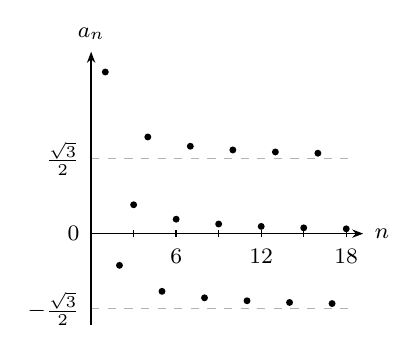
\begin{tikzpicture}[
  x=0.18cm,y=1.1cm,font=\footnotesize,line width=0.5pt,
  every node/.style={inner sep=0pt},
  >={Stealth[length=4pt,width=3pt]}
]
  \draw[gray!60,dashed] (0,{sqrt(3)/2}) -- (18.6,{sqrt(3)/2});
  \draw[gray!60,dashed] (0,{-sqrt(3)/2}) -- (18.6,{-sqrt(3)/2});
  \draw[->] (0,-1.05) -- (0,2.1) node[above=4pt] {$a_n$};
  \draw[->] (0,0) -- (19.2,0) node[right=4pt] {$n$};
  \node[left=4pt] at (0,0) {$0$};
  \node[left=4pt] at (0,{sqrt(3)/2}) {$\frac{\sqrt{3}}{2}$};
  \node[left=4pt] at (0,{-sqrt(3)/2}) {$-\frac{\sqrt{3}}{2}$};
  \foreach \n in {3,6,9,12,15,18} {
    \draw (\n,0.04) -- (\n,-0.04);
  }
  \foreach \n in {6,12,18} {
    \node[below=4pt] at (\n,-0.04) {$\n$};
  }
  \foreach \n in {1,...,18} {
    \fill (\n,{1/\n+sin(120*\n)}) circle[radius=1.25pt];
  }
\end{tikzpicture}

    \caption[Three subsequence limits.]{The first eighteen terms. The dashed lines mark
      $\pm\sqrt{3}/2$; the horizontal axis marks the third limit, $0$.}
    \label{fig:hw03:oscillating-sequence}
  \end{marginfigure}

  To show that there are no other limit points, suppose a subsequence
  converges to $\ell$. Among its infinitely many indices, at least
  one remainder occurs infinitely often. Keeping only those indices
  gives a further subsequence of one of the three sequences above.
  It still converges to $\ell$, so uniqueness of limits forces $\ell$
  to be $0$, $h$, or $-h$. Thus the set of all limit points is
  \[
    \left\{-\frac{\sqrt{3}}{2},0,\frac{\sqrt{3}}{2}\right\}.
  \]

  To find the lower limit, fix a tail beginning at $N\geq1$. Every
  term in this tail is greater than $-h$, while terms with indices
  $3k+2$ occur arbitrarily far out and approach $-h$. Therefore
  \[
    \inf\{a_n\mid n\geq N\}=-h.
  \]
  For the upper limit, every term in this tail satisfies
  $a_n\leq h+1/N$. The tail also contains terms with indices $3k+1$,
  all of which exceed $h$. Hence
  \[
    h\leq\sup\{a_n\mid n\geq N\}\leq h+\frac{1}{N}.
  \]
  Taking the limits of these tail bounds gives
  \[
    \liminf_{n\to\infty}a_n=-\frac{\sqrt{3}}{2},\qquad
    \limsup_{n\to\infty}a_n=\frac{\sqrt{3}}{2}.
  \]
\end{proof}


% !TEX root = ../../hw03.tex
% Source: HW3 Intro to Math Analysis I (1).pdf, page 1, question 4.
% "Increasing" in part (a) is non-strict, since F_1 = F_2 = 1.
\begingroup
\renewcommand{\labelenumi}{(\alph{enumi})}
\begin{exercise}
  \label{ex:hw03:fibonacci-ratios}
  The Fibonacci sequence $\{F_n\}$ is defined by
  \[
    F_0=0,\quad F_1=1,\quad F_n=F_{n-2}+F_{n-1},
    \qquad n=2,3,\ldots.
  \]
  \begin{enumerate}
    \item Show that $\{F_n\}$ is an increasing sequence.
      \emph{Here increasing means nondecreasing.}
    \item Show that $\{F_n\}$ is unbounded.
    \item Show that the Fibonacci ratios
      \[
        r_n=\frac{F_n}{F_{n-1}},\qquad n=2,3,\ldots,
      \]
      is a bounded sequence.
    \item Assume the limit of $\{r_n\}$ exists. Find the limit
      (which happens to be the golden ratio).
  \end{enumerate}
  \solutionlink{hw03:fibonacci-ratios}
\end{exercise}
\endgroup

% !TEX root = ../../hw03.tex
% Homework 03, question 4.
\begin{proof}[Solution]
  For part (a), the initial values and the recurrence show by induction
  that $F_n\geq0$ for every $n\geq0$, and $F_n\geq1$ for every
  $n\geq1$. For $n\geq1$, the recurrence gives
  \[
    F_{n+1}-F_n=F_{n-1}\geq0.
  \]
  Together with $F_1\geq F_0$, this proves that the sequence is
  nondecreasing. It is strictly increasing from $F_2$ onward, since
  $F_{n-1}>0$ when $n\geq2$. The only repeated adjacent values are
  $F_1=F_2=1$.

  % This proof could be much clearer
  % For part (b), we have $F_{n+1}\geq F_n+1$ whenever $n\geq2$.
  % Starting from $F_2=1$, induction therefore gives
  % \[
  %   \forall n\geq2,\quad F_n\geq n-1.
  % \]
  % Given any real number $M$, the Archimedean property supplies an
  % integer $n\geq2$ with $n-1>M$. Then $F_n>M$, so the sequence is
  % unbounded above.

  For part (b), suppose $(F_n)$ is bounded above. Since it is nondecreasing,
  the monotone convergence theorem gives $F_n\to L$ as $n\to\infty$.
  The shifted sequences $F_{n-1}$ and $F_{n-2}$ also tend to $L$, so the
  recurrence and the limit laws give
  \begin{align*}
    F_n&=F_{n-1}+F_{n-2} \\
       &\implies L=2L \\
       &\iff L=0.
  \end{align*}
  But $F_n\geq1$ for every $n\geq1$, so taking limits gives $L\geq1$.
  This contradicts $L=0$. Therefore the sequence is unbounded above.

  For part (c), the ratios are well defined because their denominators
  are positive. We have $r_2=1$. For $n\geq3$, substitute the recurrence
  into the numerator and split the fraction to obtain
  \begin{align*}
    r_n&=\frac{F_n}{F_{n-1}}\\
       &=\frac{F_{n-1}+F_{n-2}}{F_{n-1}}\\
       &=\frac{F_{n-1}}{F_{n-1}}+\frac{F_{n-2}}{F_{n-1}}\\
       &=1+\frac{F_{n-2}}{F_{n-1}}.
  \end{align*}
  By part (a), we have $0<F_{n-2}\leq F_{n-1}$. Dividing by the
  positive number $F_{n-1}$ gives
  \[
    0<\frac{F_{n-2}}{F_{n-1}}\leq1.
  \]
  Adding $1$ now gives $1<r_n\leq2$.
  Including $r_2$, we conclude that
  \[
    \forall n\geq2,\quad 1\leq r_n\leq2.
  \]
  Thus the ratio sequence is bounded.

  For part (d), assume that $r_n\to L$. The bounds above give
  $1\leq L\leq2$, so $L$ is nonzero.
  \begin{marginfigure}
    \centering
    % Equal axis units preserve the geometry of the diagonal.
% Curve labels sit in a separate legend so the intersection has clear space.
\begin{tikzpicture}[interval diagram,x=12mm,y=12mm]
  \pgfmathsetmacro{\goldenratio}{(1+sqrt(5))/2}

  \draw[->] (0,0) -- (2.8,0)
    node[right=4pt,interval label] {$x$};
  \draw[->] (0,0) -- (0,3.3)
    node[above=4pt,interval label] {$y$};
  \node[below left=4pt,interval label] at (0,0) {$0$};

  \draw[gray!65,densely dotted]
    (\goldenratio,0) -- (\goldenratio,\goldenratio)
    -- (0,\goldenratio);
  \draw (\goldenratio,-2pt) -- (\goldenratio,2pt);
  \draw (-2pt,\goldenratio) -- (2pt,\goldenratio);
  \node[below=5pt,interval label] at (\goldenratio,0) {$\varphi$};
  \node[left=5pt,interval label] at (0,\goldenratio) {$\varphi$};

  \draw[gray!55,dashed,->] (0,0) -- (2.55,2.55);
  \draw[<->,domain=0.46:2.55,samples=80]
    plot (\x,{1+1/\x});
  \fill (\goldenratio,\goldenratio) circle[radius=1.6pt];

  \draw[gray!55,dashed] (0,-0.75) -- (0.45,-0.75);
  \node[anchor=west,interval label] at (0.65,-0.75) {$y=x$};
  \draw (0,-1.3) -- (0.45,-1.3);
  \node[anchor=west,interval label] at (0.65,-1.3) {$y=1+1/x$};
\end{tikzpicture}

    \caption[The golden ratio as a fixed point.]{The positive intersection
      satisfies $\varphi=1+1/\varphi$. Dotted guides locate both coordinates
      at $\varphi\approx1.618$. The axes use equal units.}
    \label{fig:hw03:golden-ratio-fixed-point}
  \end{marginfigure}
  To express $r_n$ in terms of $r_{n-1}$, recall from part (c) that,
  for $n\geq3$,
  \[
    r_n=\frac{F_n}{F_{n-1}}=1+\frac{F_{n-2}}{F_{n-1}}.
  \]
  The preceding ratio is $r_{n-1}=F_{n-1}/F_{n-2}$. Since both
  Fibonacci terms are positive, we can take its reciprocal to obtain
  \[
    \frac{1}{r_{n-1}}
      =\frac{1}{F_{n-1}/F_{n-2}}
      =\frac{F_{n-2}}{F_{n-1}}.
  \]
  Substituting this into the expression for $r_n$ gives the recurrence
  \[
    r_n=1+\frac{1}{r_{n-1}},\qquad n\geq3.
  \]
  The shifted sequence $r_{n-1}$ also tends to $L$. Since $L\neq0$,
  the limit laws give
  \[
    L=1+\frac{1}{L}.
  \]
  Geometrically, $(L,L)$ lies on both $y=x$ and $y=1+1/x$, as shown
  in \autoref{fig:hw03:golden-ratio-fixed-point}.
  Multiplying by $L$ and bringing all terms to one side gives
  \[
    L^2=L+1,\qquad L^2-L-1=0.
  \]
  The two roots are $(1+\sqrt{5})/2$ and $(1-\sqrt{5})/2$.
  The second is negative and cannot satisfy $L\geq1$. Therefore the
  assumed limit is the golden ratio
  \[
    L=\frac{1+\sqrt{5}}{2}=\varphi\approx1.6180339887.
  \]
\end{proof}

The identity $\varphi-1=1/\varphi$ also has a geometric interpretation.
\begin{marginfigure}
  \centering
  % A golden rectangle and its recursive square subdivision.
% The black curve is a logarithmic golden spiral, not circular arcs.
% Geometry reference: https://doi.org/10.1155/2019/3149602
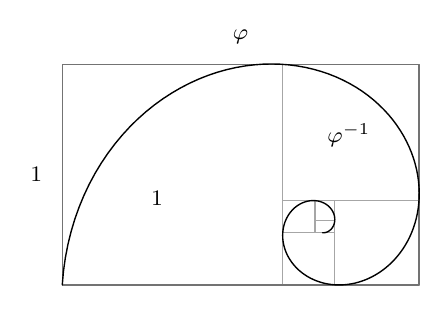
\begin{tikzpicture}[interval diagram,x=28mm,y=28mm]
  \pgfmathsetmacro{\goldenratio}{(1+sqrt(5))/2}
  \pgfmathsetmacro{\shrink}{1/\goldenratio}
  \pgfmathsetmacro{\eyex}{\goldenratio/(1+\shrink^2)}
  \pgfmathsetmacro{\eyey}{\shrink^2/(1+\shrink^2)}

  % A clockwise quarter-turn and contraction reproduce the next square.
  \foreach \step in {0,...,5} {
    \pgfmathsetmacro{\factor}{\shrink^\step}
    \pgfmathsetmacro{\turn}{-90*\step}
    \begin{scope}[
      shift={(\eyex,\eyey)},rotate=\turn,scale=\factor,
      shift={(-\eyex,-\eyey)}
    ]
      \draw[black!35] (0,0) rectangle (1,1);
    \end{scope}
  }
  \draw[black!55] (0,0) rectangle (\goldenratio,1);

  % Contract continuously while turning clockwise around the same centre.
  \draw[domain=0:630,samples=220,variable=\angle]
    plot (
      {\eyex+\shrink^(\angle/90)*
        (-\eyex*cos(\angle)-\eyey*sin(\angle))},
      {\eyey+\shrink^(\angle/90)*
        (\eyex*sin(\angle)-\eyey*cos(\angle))}
    );

  % Only label the two largest squares; leave the inner turns uncluttered.
  \node[interval label] at (0.43,0.39) {$1$};
  \node[interval label] at (1.3,0.68) {$\varphi^{-1}$};
  \node[above=6pt,interval label] at (\goldenratio/2,1) {$\varphi$};
  \node[left=6pt,interval label] at (0,0.5) {$1$};
\end{tikzpicture}

  \caption[The golden rectangle and golden spiral.]{A golden rectangle
    subdivides into squares with side lengths
    $1,\varphi^{-1},\varphi^{-2},\ldots$. The golden spiral passes through
    successive corners. Each quarter-turn inward shrinks the distance
    from its centre by $1/\varphi$. The subdivision continues indefinitely.}
  \label{fig:hw03:golden-rectangle-spiral}
\end{marginfigure}
A rectangle with side lengths $1$ and $\varphi$ leaves a smaller,
rotated copy of itself when a unit square is removed. Repeating this
step gives the squares in \autoref{fig:hw03:golden-rectangle-spiral}.
The golden spiral winds through their corners, shrinking its distance
from the centre by $1/\varphi$ with each
quarter-turn~\cite{Duan2019GoldenSpirals}.


% !TEX root = ../../hw03.tex
% Source: HW3 Intro to Math Analysis I (1).pdf, page 2, question 5.
% The source's quoted terms "sparse" and "incompleteness" are retained.
% Small covering length alone is not a criterion for metric incompleteness.
\begingroup
\renewcommand{\labelenumi}{(\alph{enumi})}
\begin{exercise}
  \label{ex:hw03:rational-interval-cover}
  Let the rational numbers in $[0,1]$ be enumerated by
  $q_0,q_1,\ldots,q_n,\ldots$. Let $\varepsilon>0$ and cover this set
  $Q=\{q_n\}$ by
  \[
    U_\varepsilon=\bigcup_{n=0}^{\infty}I_n(\varepsilon),
  \]
  \[
    I_n(\varepsilon)=(q_n-\varepsilon 2^{-n},q_n+\varepsilon 2^{-n}),
    \qquad n=0,1,2,\ldots.
  \]
  That is, $Q\subset U_\varepsilon$.
  \begin{enumerate}
    \item Show that the sum of the lengths of the intervals
      $\{I_n(\varepsilon)\}$ satisfies the bound
      \[
        \sum_{n=0}^{\infty}|I_n(\varepsilon)|\leq4\varepsilon.
      \]
    \item Since $\varepsilon>0$ can be arbitrarily small, the set $Q$ can
      be covered by intervals of arbitrarily small total length indicating
      that $Q$ is a rather ``sparse'' subset of $[0,1]$. In view of this
      fact, give your explanation regarding the ``incompleteness'' of $Q$
      in $[0,1]$.
  \end{enumerate}
  \solutionlink{hw03:rational-interval-cover}
\end{exercise}
\endgroup

% !TEX root = ../../hw03.tex
% Homework 03, question 5. No solution supplied yet.
\noindent\emph{Awaiting solution.}


% !TEX root = ../../hw03.tex
% Source: HW3 Intro to Math Analysis I (1).pdf, page 2, question 6.
\begingroup
\renewcommand{\labelenumi}{(\alph{enumi})}
\begin{exercise}
  \label{ex:hw03:rational-exponent-laws}
  For $x\in\R_+$, we defined the function $x^{1/n}$ for $n\in\N$.
  \begin{enumerate}
    \item For $x,y\in\R_+$, prove that $(xy)^{1/n}=x^{1/n}y^{1/n}$.
    \item For $x\in\R_+$, we defined $x^{m/n}=(x^m)^{1/n}$ for
      $m\in\N$. Show that this is the same as $(x^{1/n})^m$.
    \item For $x\in\R_+$ and $r,s\in\Q_+$, prove the laws of exponents
      \[
        (x^r)^s=x^{rs},\qquad x^{r+s}=x^rx^s.
      \]
  \end{enumerate}
  \solutionlink{hw03:rational-exponent-laws}
\end{exercise}
\endgroup

% !TEX root = ../../hw03.tex
% Homework 03, question 6.
\begin{proof}[Solution]
  We use $\R_+=[0,\infty)$ and positive rational exponents. The
  nonnegative $n$th root exists and is unique for every positive
  integer $n$.

  For part (a), put $u=x^{1/n}$ and $v=y^{1/n}$. Both are nonnegative,
  and the integer power laws give
  \[
    (uv)^n=u^nv^n=xy.
  \]
  Thus $uv$ is the nonnegative $n$th root of $xy$. Uniqueness gives
  \[
    (xy)^{1/n}=x^{1/n}y^{1/n}.
  \]

  For part (b), put $w=(x^{1/n})^m$. This number is nonnegative, and
  \[
    w^n=(x^{1/n})^{mn}=\bigl((x^{1/n})^n\bigr)^m=x^m.
  \]
  Hence $w$ is the nonnegative $n$th root of $x^m$. Again by
  uniqueness,
  \[
    x^{m/n}=(x^m)^{1/n}=(x^{1/n})^m.
  \]

  For part (c), write $r=m/n$ and $s=p/q$, where $m,n,p,q$ are
  positive integers. We use the fact that rational powers are
  independent of the fraction used to represent the exponent.
  First let $u=(x^r)^s$. By definition, $u\geq0$ and
  $u^q=(x^r)^p$. Taking integer powers gives
  \[
    u^{nq}=\bigl((x^r)^p\bigr)^n
      =\bigl((x^r)^n\bigr)^p=x^{mp}.
  \]
  Since $rs=mp/(nq)$, the number $x^{rs}$ is also the nonnegative
  $(nq)$th root of $x^{mp}$. Therefore
  \[
    (x^r)^s=x^{rs}.
  \]

  For the sum law, let $v=x^rx^s$. This is nonnegative, and
  \begin{align*}
    v^{nq}
      &=(x^r)^{nq}(x^s)^{nq} \\
      &=\bigl((x^r)^n\bigr)^q\bigl((x^s)^q\bigr)^n \\
      &=x^{mq}x^{pn}=x^{mq+pn}.
  \end{align*}
  But $r+s=(mq+pn)/(nq)$, so $x^{r+s}$ is the nonnegative $(nq)$th
  root of the same number. Uniqueness therefore gives
  \[
    x^{r+s}=x^rx^s.
  \]
  These arguments include $x=0$, since all exponents are positive
  and we never divide by $x$.
\end{proof}


% !TEX root = ../../hw03.tex
% Source: HW3 Intro to Math Analysis I (1).pdf, page 2, question 7.
\begin{exercise}
  \label{ex:hw03:reverse-triangle-inequality}
  Use the triangle inequality to prove
  \[
    \bigl||x|-|y|\bigr|\leq|x-y|,\qquad x,y\in\R.
  \]
  When will this become an equality?
  \solutionlink{hw03:reverse-triangle-inequality}
\end{exercise}

% !TEX root = ../../hw03.tex
% Homework 03, question 7.
\begin{proof}[Solution]
  Write $x=(x-y)+y$. The triangle inequality gives
  \[
    |x|\leq|x-y|+|y|,
  \]
  and therefore $|x|-|y|\leq|x-y|$. Interchanging $x$ and $y$ gives
  $|y|-|x|\leq|y-x|=|x-y|$. Combining the two inequalities, we obtain
  \[
    -|x-y|\leq|x|-|y|\leq|x-y|.
  \]
  This is exactly
  \[
    \bigl||x|-|y|\bigr|\leq|x-y|.
  \]

  For equality, first suppose $xy\geq0$. If both numbers are
  nonnegative, then
  \[
    \bigl||x|-|y|\bigr|=|x-y|.
  \]
  If both are nonpositive, then $|x|=-x$ and $|y|=-y$, so
  \[
    \bigl||x|-|y|\bigr|=|-x+y|=|x-y|.
  \]
  These cases also include either number being zero.

  If $xy<0$, the numbers have opposite signs and neither is zero.
  Then $|x-y|=|x|+|y|$. Since both $|x|$ and $|y|$ are positive,
  \[
    \bigl||x|-|y|\bigr|<|x|+|y|=|x-y|.
  \]
  Thus equality holds exactly when $xy\geq0$. Taking absolute values
  can be pictured as folding the number line at zero. Points on the
  same side keep their separation, while points on opposite sides
  move closer together. \autoref{fig:hw03:reverse-triangle-distance}
  illustrates this folding.
  \begin{marginfigure}
    \centering
    % Original folding analogy for the reverse triangle inequality.
% Background on absolute value as distance from zero and geometric inequalities:
% https://danaernst.com/IntroToProofViaIBL/sec_AxiomsRealNumbers.html
% Both rows use the same scale; the illustrated case is y < 0 < x < |y|.
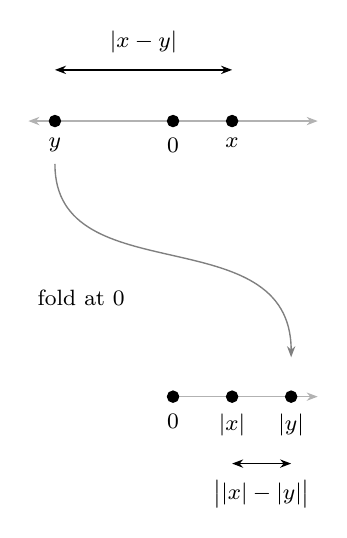
\begin{tikzpicture}[interval diagram,x=7.5mm,y=1cm]
  \draw[<->,gray!60] (-2.45,0) -- (2.45,0);
  \foreach \position/\name in {-2/y,0/0,1/x} {
    \node[interval closed] at (\position,0) {};
    \node[interval label,below=5pt] at (\position,0) {$\name$};
  }
  \draw[<->] (-2,0.65) -- (1,0.65)
    node[midway,above=5pt,interval label] {$|x-y|$};

  % Move the negative point onto the positive half-line without crossing
  % either distance arrow. Keep the annotation in the open part of the bend.
  \draw[->,gray] (-2,-0.55)
    .. controls (-2,-2.2) and (2,-1.2) .. (2,-3.0);
  \node[interval label,anchor=west] at (-2.35,-2.25) {fold at $0$};

  \draw[->,gray!60] (0,-3.5) -- (2.45,-3.5);
  \foreach \position/\name in {0/0,1/{|x|},2/{|y|}} {
    \node[interval closed] at (\position,-3.5) {};
    \node[interval label,below=5pt] at (\position,-3.5) {$\name$};
  }
  \draw[<->] (1,-4.35) -- (2,-4.35)
    node[midway,below=5pt,interval label] {$\bigl||x|-|y|\bigr|$};
\end{tikzpicture}

    \caption[Folding the number line at zero.]{Schematic folding by $t\mapsto|t|$.
      Both rows use the same scale. Here $y<0<x<|y|$, and the gap shrinks
      from $|x-y|$ to $\bigl||x|-|y|\bigr|$. Points on the same half-line
      keep their separation.}
    \label{fig:hw03:reverse-triangle-distance}
  \end{marginfigure}
\end{proof}


% !TEX root = ../../hw03.tex
% Source: HW3 Intro to Math Analysis I (1).pdf, page 2, question 8.
\begin{exercise}
  \label{ex:hw03:odd-roots}
  Show that for $n=3,5,7,\ldots$, the function $x^{1/n}$ is a well-defined
  monotone increasing function which is a bijection from $\R$ to itself.
  (Hint: Study $x^n$ as we did in class.)
  \solutionlink{hw03:odd-roots}
\end{exercise}

% !TEX root = ../../hw03.tex
% Homework 03, question 8. No solution supplied yet.
\noindent\emph{Awaiting solution.}


\analysisbibliography

\end{document}
